\documentclass[8pt, a4paper]{article}
\usepackage{geometry}
\geometry{total={170mm, 257mm},left=20mm, top=20mm}
\usepackage{graphicx}
\usepackage{hyperref}

\begin{document}
\setlength \topmargin{-1in}
\title{\textbf{Software Engineering for Distributed and Interactive Systems.}}
\author{\textbf{James Ravenhill}}
\date{}
\maketitle

\section{Introduction} 

The main outcome at the beginning of the project was to create a simple and easy to used piece of software which allows the user to control the buggy without being too complex. Both the hardware and software have been an ongoing development based on feedback given through multiple tests, which a few friends generously took part in. The main objectives of the project are listed below but not limited to:

\begin{itemize}
	\item Reliability - Unreliable connection/data transfer is a disadvantage and creates more problems. This will be explained later in more detail.  
	\item  Multiple methods of communication - By using WiFi, Bluetooth, IR remote and PC. 
	\item Scalability - There should be no software problems while developing the increased load of sensor/capabilities of the buggy. 
	\item Maintainability - comments/documentation is clear to allow future developers to understand the project decisions as they happen.  
\end{itemize}

In this document short snips of the main code will be used in explanations. The main raw code can be found in the submitted documents or on my $\href{https://github.com/james8268/Buggy}{Github}$ account.
 

\section{Design}
In terms of hardware design, the overall aesthetic is not very relevant. This being said, proper cable management and reducing the risk of damaging hardware was a great challenge due to the limited mounting points on the buggy. This challenge was overcome by using blue tac or Velcro to attach the hardware to the buggy without damaging the hardware in the process. 

///////insert two pics of the buggy.  


Below are two images of the main schematic of the buggy and a general communications diagram. 
\begin{figure}[h]
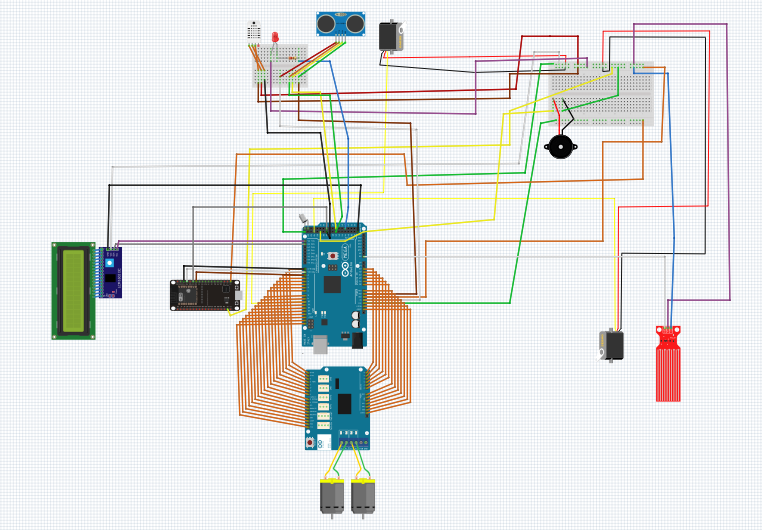
\includegraphics[height=5cm, width=7.0cm]{schematic}
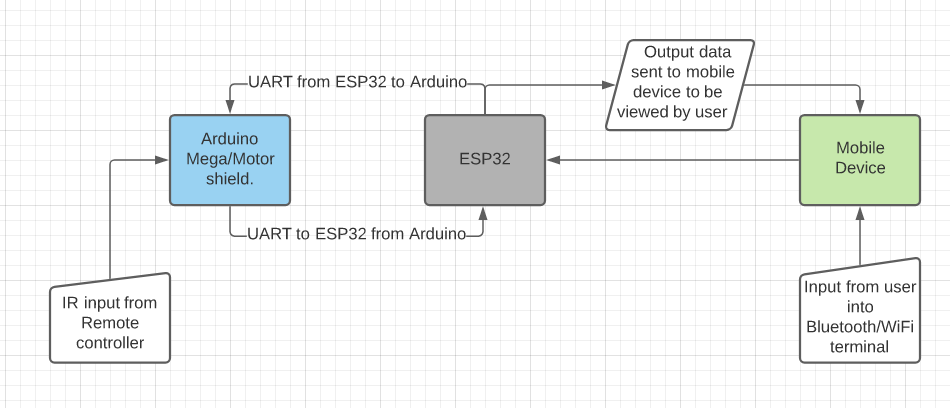
\includegraphics[height=5cm, width=7.0cm]{Arch}
\caption{Left: Schematic of Buggy.}
\caption{Right: communication graph of the Buggy}
\end{figure}

The software for the Ardunio has been set up into header (.h) files and source code (.cpp) files where they are then called in the main code. There are many benefits to this such as the code is organised and tidy allowing future and current developers to debug with ease, addition of any new code can be easily integrated into the system and the code can be easily maintained. 

//// add image of arduino tabs.


The software for the ESP32 comprised of individual sketch files which correspond to the use of WiFi or Bluetooth and for both due to the ESP32 being dual-core. Transmission control protocol (TCP) has been used when using WiFi instead of user diagram protocol (UDP) as is it more reliable, has Flow control so will not overwhelm reciever and has congestion control. A 'handshake' is used to initiate communication and then multiple packets are sent. TCP may not be as fast as UDP but due to the project objectives, reliability is preferred. This being said TCP is slower by a very small margin so is not a large hindrance on the usability of the system. 
 
 


/////talk about design of distributed and interactivity. 

At the start of the project when the polarity of the motors for the wheels was established I wanted to included an LCD screen using the I2C bus. This then allowed testing/setup of the ultrasound sensor to be more convenient while driving the buggy (while not attached to a PC). The LCD screen is then used later on to provide security start up messages e.g. Present RFID tag. It also allows the use of the IR remote while still being able to receive visual temperature, humidity and water level data.  


\section{Implementation}


\section{Testing}

\section{Evaluation}


\section{Code quality/remarks} ////this may get cut if needed as in more an non written task
////discuss multi and single core methods in a ReadMe file!!!


///Layers- layered system to allow for easy maintenance, ease of updating/developing the system. ADD A DIAGRAM OF THE LAYERS HERE. 


\section{Demonstration}
////film the video and then refer to it for the following subsections


\subsection{Distribution}
///Define what a distributed system is 

\subsection{Interactive}
///Define what an interactive system is

\subsection{Performance}






\section{Conclusion}


\section{Reference Library and appendices}
\subsection{Github account}

\href{https://github.com/james8268/Buggy}{Click here for Github hyper link} 

or copy and paste the URL into your web browser. https://github.com/james8268/Buggy

\listoffigures

\end{document}